\documentclass[tikz,border=5pt]{standalone}
\usepackage{tikz}
\usepackage{amsmath}

\begin{document}

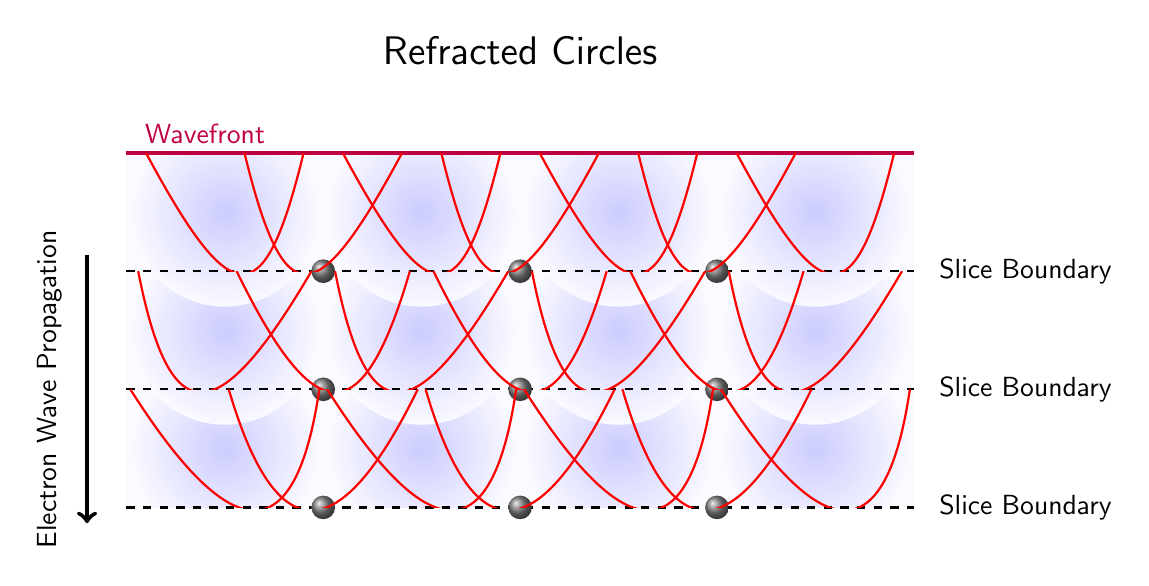
\begin{tikzpicture}[font=\sffamily]
    % Define coordinates for the planes
    \coordinate (TopPlaneLeft) at (0, 3);
    \coordinate (TopPlaneRight) at (10, 3);
    \coordinate (MidPlaneLeft) at (0, 1.5);
    \coordinate (MidPlaneRight) at (10, 1.5);
    \coordinate (BotPlaneLeft) at (0, 0);
    \coordinate (BotPlaneRight) at (10, 0);

    % Title
    \node[anchor=south] at (5, 5.5) {\Large Refracted Circles};

    % Visualize the continuous potential / refractive index
    % Using generic blobs/gradients to show the medium is "filled"
    \fill[blue!2] (0,0) rectangle (10, 4.5);
    
    % Add potential variations (blobs) to represent varying refractive index
    \begin{scope}
        \clip (0,0) rectangle (10, 4.5);
        \foreach \x in {1.25, 3.75, 6.25, 8.75} {
            \foreach \y in {0.75, 2.25, 3.75} {
                 \shade[inner color=blue!20, outer color=blue!2] (\x, \y) circle (1.2);
            }
        }
    \end{scope}

    % Draw Slice Boundaries
    \foreach \y in {0, 1.5, 3} {
        \draw[thick, black, dashed] (0,\y) -- (10,\y);
        \node[anchor=west] at (10.2, \y) {Slice Boundary};
        % Add some scattering centers on the boundary
        \foreach \x in {2.5, 5, 7.5} {
            \shade[ball color=gray] (\x, \y) circle (0.15);
        }
    }

    % Electron Wave Propagation Arrow
    \draw[->, ultra thick, black] (-0.5, 3.2) -- (-0.5, -0.2);
    \node[rotate=90, anchor=south, black] at (-0.7, 1.5) {Electron Wave Propagation};
    
    % Initial Wavefront line
    \draw[ultra thick, purple] (0, 4.5) -- (10, 4.5);
    \node[purple, anchor=south] at (1, 4.5) {Wavefront};

    % Spherical Wavefronts (WPM)
    % Detailed: Distorted curves starting from top of slice, curving down to touch bottom
    % Introduced randomness/shifts in control points to simulate index variation

    % 1. Between y=4.5 and y=3
    \begin{scope}
        \clip (0, 3) rectangle (10, 4.5);
        \foreach \x [count=\i] in {1.25, 2.5, 3.75, 5.0, 6.25, 7.5, 8.75} {
             % Introduce a shift based on index (even/odd) to look distorted
             \pgfmathsetmacro{\xshift}{isodd(\i) ? 0.3 : -0.3}
             \draw[thick, red] (\x-1.0, 4.5) .. controls (\x+\xshift-0.2, 2.45) and (\x+\xshift+0.2, 2.45) .. (\x+1.0, 4.5);
        }
    \end{scope}
    
    % 2. Between y=3 and y=1.5
    \begin{scope}
        \clip (0, 1.5) rectangle (10, 3);
        \foreach \x [count=\i] in {1.25, 2.5, 3.75, 5.0, 6.25, 7.5, 8.75} {
             % Different shift pattern
             \pgfmathsetmacro{\xshift}{isodd(\i) ? -0.4 : 0.2}
             \draw[thick, red] (\x-1.1, 3.0) .. controls (\x+\xshift-0.3, 0.95) and (\x+\xshift+0.3, 0.95) .. (\x+1.1, 3.0);
        }
    \end{scope}
    
    % 3. Between y=1.5 and y=0
    \begin{scope}
        \clip (0, 0) rectangle (10, 1.5); 
        \foreach \x [count=\i] in {1.25, 2.5, 3.75, 5.0, 6.25, 7.5, 8.75} {
             % More extreme shift
             \pgfmathsetmacro{\xshift}{isodd(\i) ? 0.5 : -0.2}
             \draw[thick, red] (\x-1.2, 1.5) .. controls (\x+\xshift-0.4, -0.55) and (\x+\xshift+0.4, -0.55) .. (\x+1.2, 1.5);
        }
    \end{scope}

\end{tikzpicture}

\end{document}
